\subparagraph*{Submission : }
\textit{Consider the case in which prices are fixed, but the assignment of promos to users need to be optimized by using an assignment algorithm. All the parameters need to be learnt.}\\

The problem requires to optimize the assignment of the problem using an assignment algorithm, in the following scenario:
\begin{itemize}
	\item The prices are fixed
	\item All the parameter need to be learnt
\end{itemize}

\subsection*{Basic knowledge}
DIRE CHE BANDIT PROBLEM è e RIVEDERE SE QUELLI PRECEDENTI SONO GIUSTI. AGGIUNGERE UN PO' DI TEORIA
\subparagraph*{UCB Matching}
Pseudocode\\
At $t$, play a superarm $a_{t}$ such that:\\
$a_{t} \leftarrow \argmax\limits_{\textbf{a} \in M}{\left\{\sum\limits_{a \in \textbf{a}}\bar{x}_{a,t} + \sqrt{\frac{2 log(t)}{{n_{a}(t-1)}} }\right\}}$ \\
where $M$ is the set of matches.

\subsection*{Strategy}

We consider a time horizon of 60 days. We simulate the randomly arrival of the customers and the purchase of the first item. In case of purchase of the first item, we retrieve the optimal matching for the user categories from the learner (UCB matching) and we propose the second item to him, at the discounted price based on the matching suggested by the learner. The learner provides us a set of arms, so we cannot update it with the reward given by the single customer. We introduce two matrixes of shape (|User category |, |Type of promo|), every cell represents the matching between a specific customer category and a specific promo.The first matrix contains the sum of the rewards for that matching, the second contains the number of occurences that the matching has been chosen. At the beginning of the simulation, we use the first 1000 samples (customers) to initialize the two matrix, forcing all the possible combinations of matching. In this way we can update the learner, customer by customer, using the average reward for every matching.
\subparagraph{Implementation} 
\subparagraph{Optimal strategy}


\subsection*{Results}
\begin{center}
	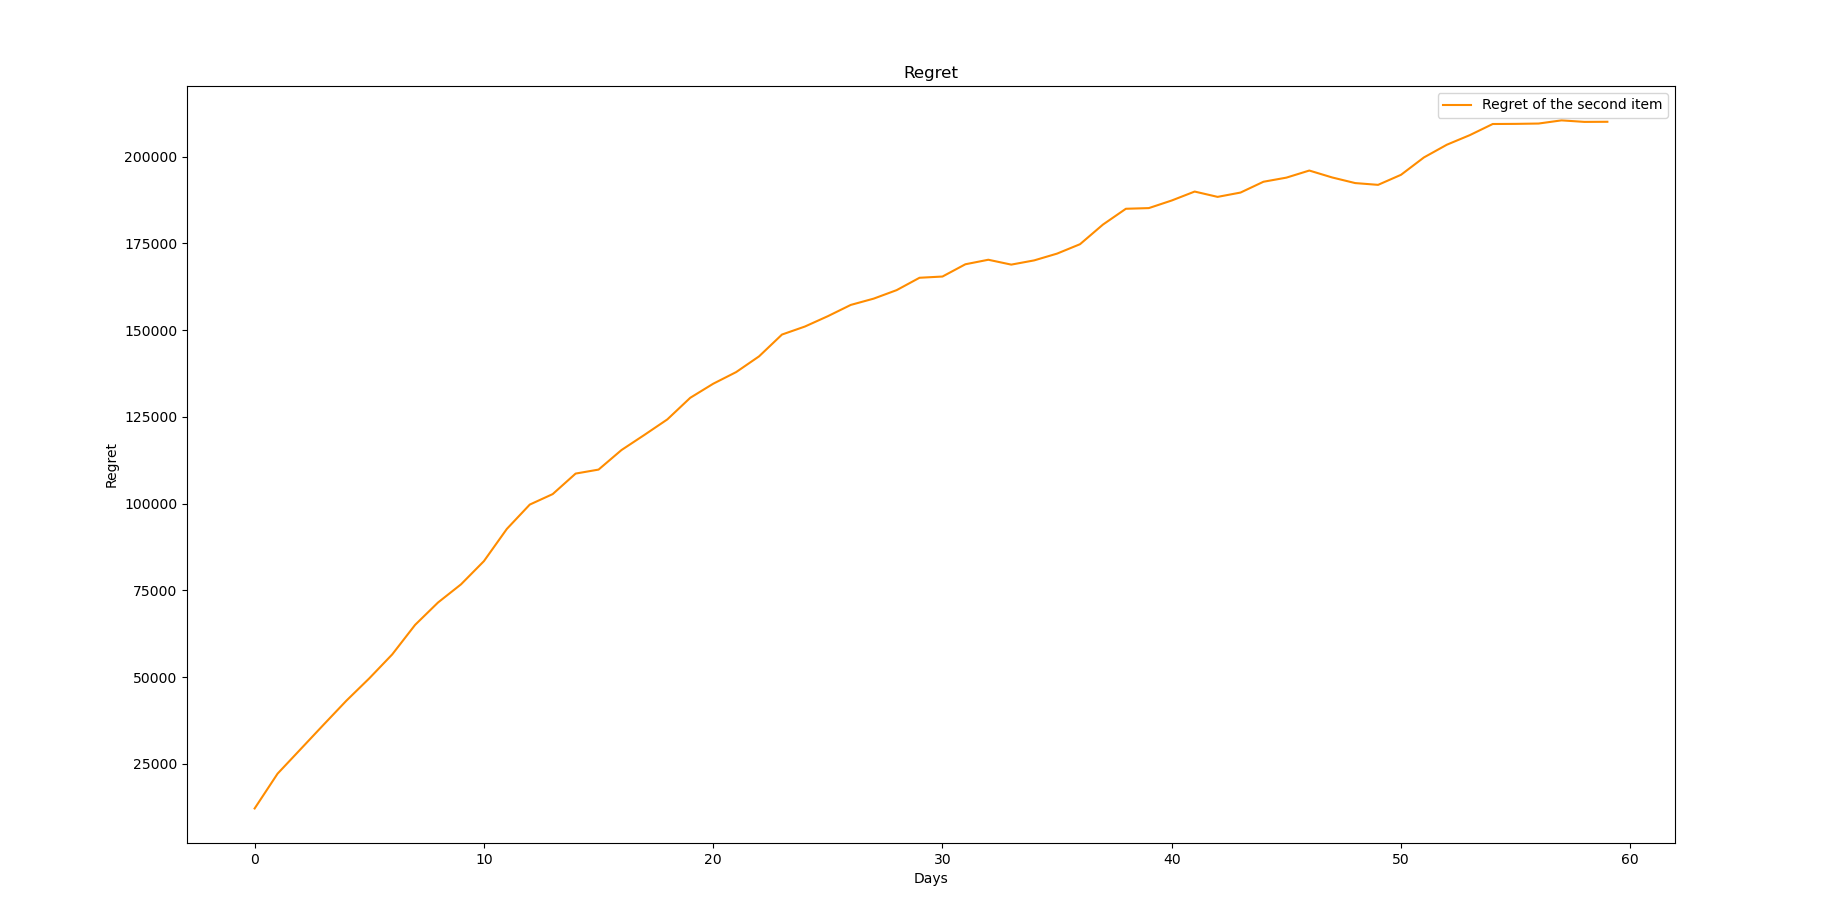
\includegraphics[scale=0.30]{Images/n5}
\end{center}
\subsection*{Considerations}
We can observe that the UCB Matching algorithm has a linear increase on the cumulative regret for the first thirty days, but after that, it becomes more and more stable on the optimal matching, and the cumulative regret does not increase so much.